\section{Datenbankschicht\label{Datenbankschicht}}
\begin{figure}[hptb]
  \begin{minipage}[b][7.5cm][t]{.5\linewidth}
Dieser Teil des Gesamtsystems setzt sich aus den Teilbereichen Datenbank, der dazu gehörigen Datenbankabstraktion und dem Dateisystem zusammen.\\

Dabei kann jedes Teilsystem unabhängig von den übrigen betrieben und erweitert werden. Eine Verknüpfung derer entsteht durch die entsprechende Konfiguration.\\

Um den Zugriff anderer Schichten auf das Dateisystem und die Daten\-bank\-abstraktion zu erleichtern, wurden hier sogenannte Controller als zentrale Zugangspunkte angelegt. Diese leiten eingehende Anfragen an die verantwortlichen Komponenten in ihren Teilbereichen weiter und sollten ausschließlich genutzt werden. 
  \end{minipage}
  \begin{minipage}[b]{.5\linewidth}
    \centering
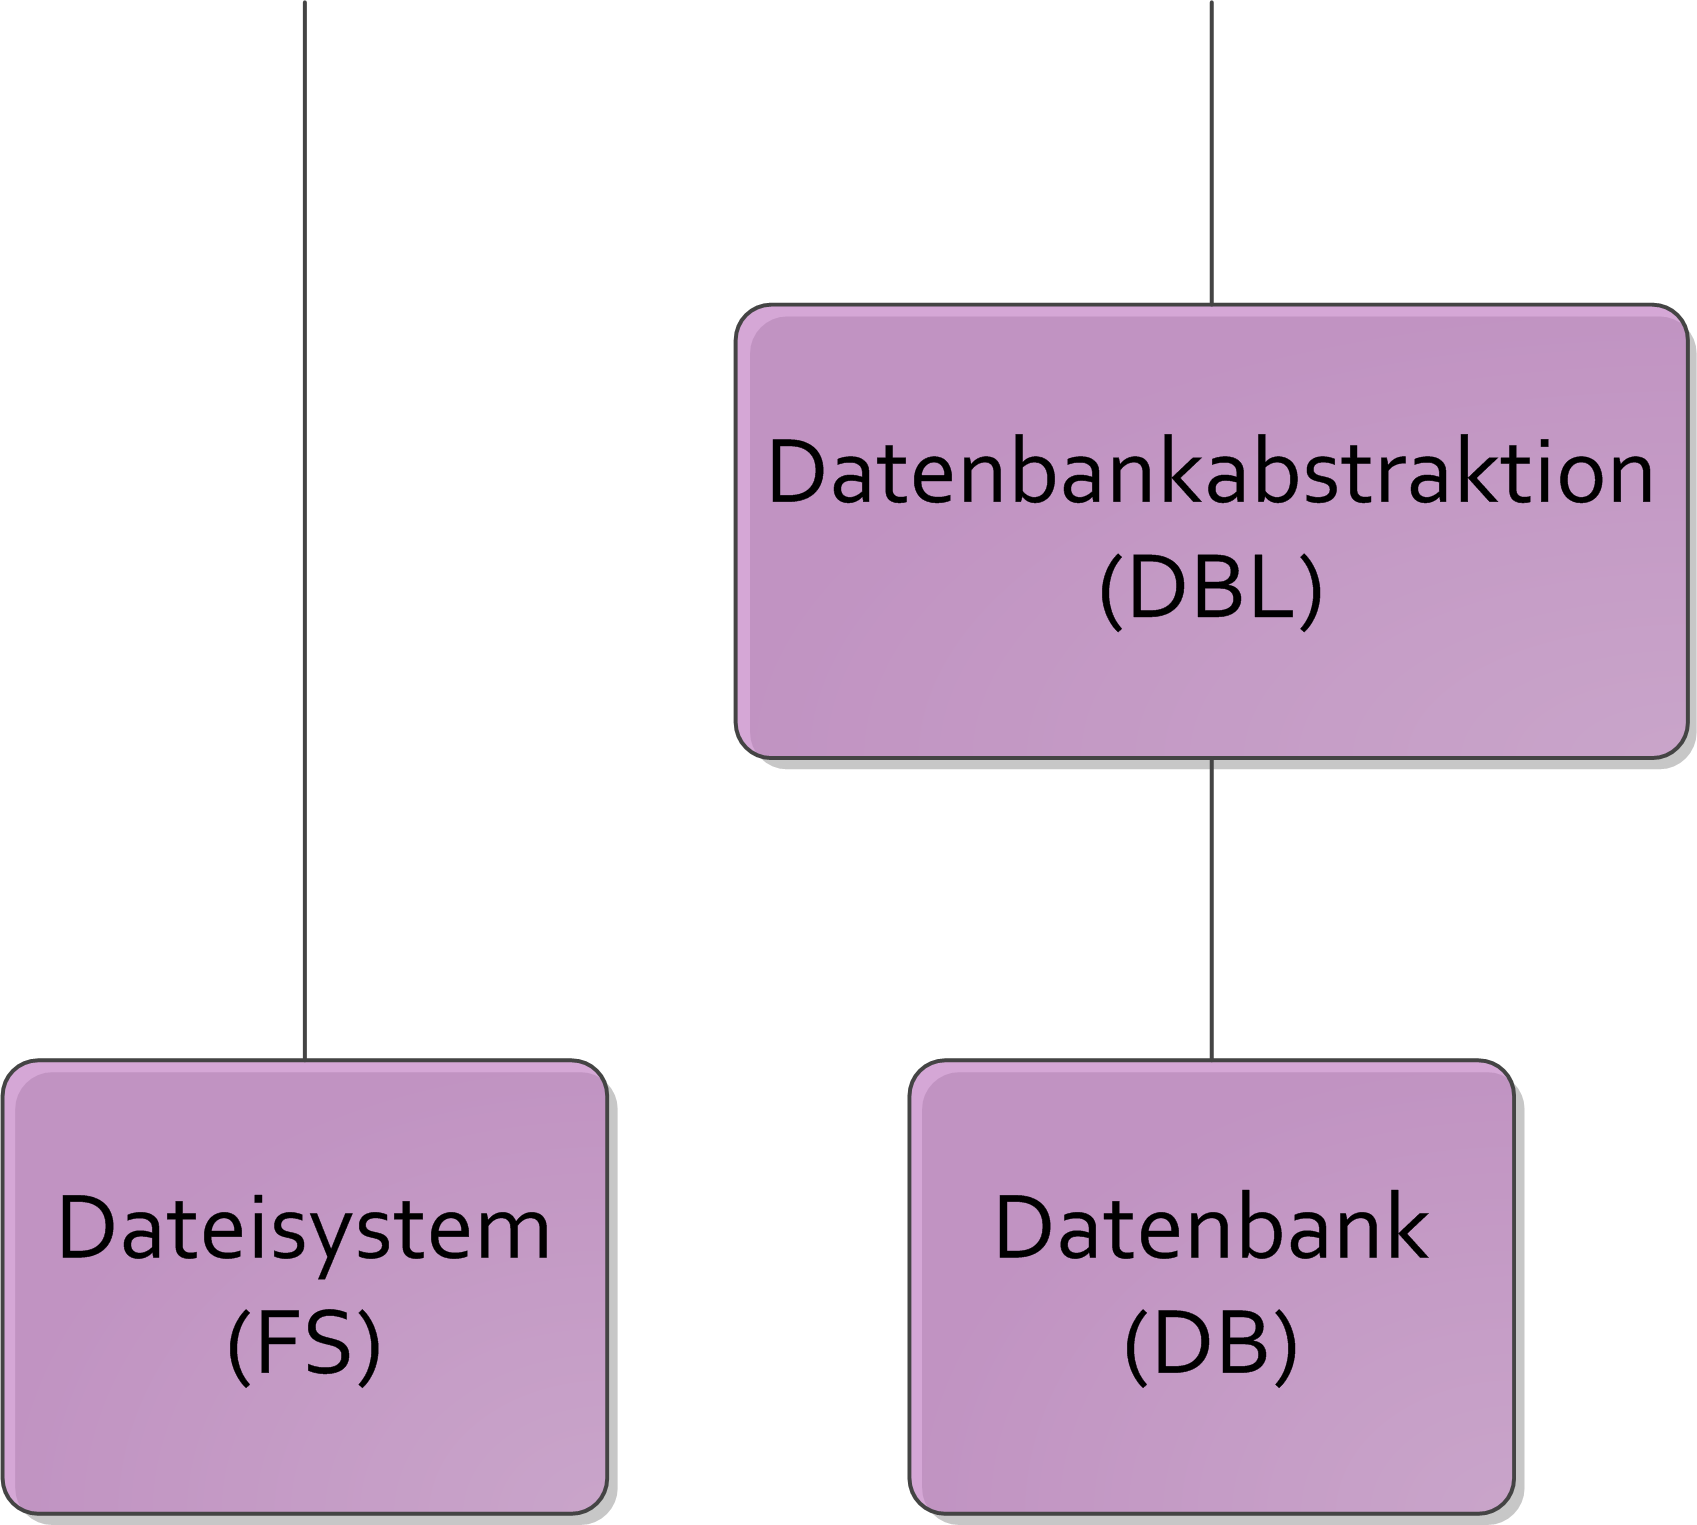
\includegraphics[scale=0.5]{Images/DB-Schichten.png}
  \end{minipage}\hfill
\end{figure}

 

\subsection{Datenbank (DB)}
\parbox{\textwidth}{Sowohl für die Speicherung der Daten, welche sich während des Betriebs der Übungsplattform ansammeln, als auch für die betriebsnotwendigen Daten wurde eine Datenbank für die Nutzung mit einem MYSQL Server unter Verwendung von MYSQL Workbench 6.0 modelliert. Dabei ergab sich ein Umfang von 19 Tabellen mit über 100 Attributen. }

\parbox{\textwidth}{Zur Beschleunigung von lesenden Anfragen wurden bei einigen Tabellen zusätzliche Attribute angelegt, wodurch die Notwendigkeit oft genutzter Join-Vorgänge minimiert wird. Der Inhalt dieser Spalten wird beim Einfügen einer neuen Datenzeile automatisch von der Datenbank mit Hilfe von implementierten Triggern befüllt, sodass diese Informationen nicht explizit angeben werden müssen.} 

\parbox{\textwidth}{Die Datenbank sollte als reiner Speicherort, ohne Wissen über den Rest des Systems, betrieben werden. Dennoch wurden aus Konsistenzgründen, zur Vereinfachung des Aufwands für andere Teilbereiche und zur Steigerung der Leistung einige Mechanismen in Form von Triggern implementiert.
Es wurden beispielsweise 35 Trigger verschiedenster Art entwickelt, um sicherzustellen, dass eine Anmeldung am System nur dann möglich ist, wenn der Nutzer nicht als gesperrt vermerkt ist.}
 
\parbox{\textwidth}{Zur Überprüfung der Langzeitstabilität des Entwurfs wurde die Datenbank während der Zeit der Entwicklung mit Beispieldaten im Umfang von rund 700.000 Datensätzen betrieben. Weiterhin wurde für eine kalkulierte Laufzeit des Systems von fünf Jahren ein lauffähiger Versuch mit über 700 Millionen Datensätzen durchgeführt.}

\parbox{\textwidth}{Zudem verwaltet die Datenbank die Verknüpfung der Komponenten der Daten\-bank\-abstraktion, des Dateisystems und der Logik-Schicht. Dafür werden ausgehende Aufrufe von Komponenten als Links bezeichnet und mit einem Namen und einer Ziel\-adresse gespeichert. Diese können dann per Aufruf über eine speziell dafür entworfene Komponente an alle im System befindlichen Komponenten verteilt werden, wodurch die zentrale Verwaltung und Konfiguration sichergestellt wird. Diese Entwurfsüberlegung ermöglicht es, das Weiterleitungsverhalten einzelner Komponenten zentral zu verändern und im Bedarfsfall zusätzliche Komponenten an entsprechenden Stellen einzuhängen, um so das System zu erweitern.}


\subsection{Datenbankabstraktion (DBL)}
\parbox{\textwidth}{Um den Zugang zur Datenbank zu vereinfachen und den direkten Zugriff über SQL Befehle zu vermeiden, wurde eine Vereinfachung entwickelt, welche feste Befehle nach außen über eine mittels Slim umgesetzte REST-API zur Verfügung stellt. Dazu wurden zusätzlich Datenstrukturen für die inhaltliche Darstellung und Kommunikation von Objekten entworfen, welche die DBL in Form eines JSON-konformen Objekts erwartet und in ihren Antworten ebenso auch kodiert.}

\parbox{\textwidth}{Die Anfragen werden nach dem Eintreffen in SQL Befehle übersetzt und mit einer der DBL zur Verfügung gestellten Datenbankschnittstelle umgesetzt.}

\parbox{\textwidth}{Dieses Vorgehen, welches direkte Datenbankzugriffe unterbindet, steigert die Austauschbarkeit sowie die einfache Erweiterbarkeit der Befehlsvielfalt. Außerdem wird an dieser Stelle sichergestellt, dass die Abfragen festgelegte Bedingungen erfüllen, wie beispielsweise die Einhaltung eines bestimmten Datentyps für Parameter des REST-Aufrufs. Darüber hinaus werden eingehende Daten von unerlaubten Inhalten bereinigt, um einen nicht ordnungsgemäßen Zugriff auf innere Systeme sowie Datenbestände zu verhindern.}

\parbox{\textwidth}{Um ein umfangreiches Angebot unterschiedlichster Anfragen an die Datenbank bereitstellen zu können, wurde ein Verbund aus 20 unabhängigen Komponenten mit über 140 Befehlen entwickelt, wobei eine  Komponente im Allgemeinen für die Bereitstellung von Funktionen zur Handhabung der entsprechenden Tabelle der Datenbank zuständig ist.}

\parbox{\textwidth}{Zur Sicherstellung der korrekten Funktionalität der Komponenten wurden einfache, automatisierte Tests unter Verwendung des PHPUnit Frameworks entworfen, durch welche die Komponenten in ihrer Gesamtheit auf die Erfüllung von über 400 Bedingungen geprüft werden können. Es muss jedoch angemerkt werden, dass diese Tests keine ausführliche Prüfung der Funktionalität der Komponenten darstellen.}

\subsection{Dateisystem (FS)}
\parbox{\textwidth}{Zur Speicherung von Dateiinhalten -- wie beispielsweise die von Studenten eingereichten Lösungen zu Übungsaufgaben -- wurden fünf weitere Komponenten entwickelt. Diese sind für die Verwaltung gespeicherter Inhalte, die Wahl des Speicherortes und der Erstellung von Archiven im ZIP-Format aus gespeicherten Inhalten zuständig. }

\parbox{\textwidth}{Es war dabei ein wesentliches Anliegen, dass die redundante Speicherung von Dateiinhalten vom Dateisystem selbstständig verhindert wird. Dies geschieht durch die Benennung der gespeicherten Dateien anhand des SHA1-Hashs, welcher von der entsprechenden Datei gebildet wird.}

\parbox{\textwidth}{Das Dateisystem behandelt die Dateiinhalte, ohne dabei die Herkunft oder die Bedeutung der Dateien kennen zu müssen. Zusätzlich ist es bereits in der Lage, die zu speichernden Inhalte per Konfiguration auf mehrere Speicherorte gleichmäßig zu verteilen, was durch die Entscheidung, einen Hash als Speichernamen zu verwenden, ermöglicht wurde.}


\subsection{Sicherheitskonzept der Datenbankschicht}
Die Datenbankschicht kann lediglich sicherstellen, dass die Informationen die eingehen, nicht dieser Schicht schaden können. Dabei kann nicht sichergestellt werden, das die Aufrufe, die an sie gestellt werden für den Nutzer erlaubt sind. Sodass jemand eine korrekte Abfrage zum Abrufen aller Nutzerdaten formulieren könnte, ohne das sich die Datenbankschicht daran stört.

\subsubsection{Datenbank}
Die SQL Anfragen, welche an der Datenbank eintreffen, müssen bereits korrekt sein und werden an dieser Stelle nicht weiter geprüft. Daher sollten Anfragen lediglich über die $DBQuery$ mithilfe der $Query$ Datenstruktur, an die Datenbank gestellt werden.

\subsubsection{Datenbankabstraktion}
Der Schutz der Datenbank vor unerlaubten Zugriffen, sowie der Ausführung nicht erlaubter Befehle wird innerhalb dieses Bereichs sichergestellt.

Dabei werden eingehende Daten für POST und PUT Zugriffe durch die \blau{getInsertData()} Funktionen der Datenstrukturen maskiert, um unerlaubte Zeichen innerhalb der Daten zu unterbinden. Dazu wird die \blau{DBJson::mysql\_real\_escape\_string()} Funktion genutzt.

\begin{minipage}{\textwidth}
\begin{lstlisting}
...
if ($this->id != null) 
    $this->addInsertData(
        $values, 
        'C_id',
        DBJson::mysql_real_escape_string($this->id));
...
\end{lstlisting}
\end{minipage}

Informationen die über die REST Aufrufe zu den Komponenenten gelangen, beispielsweise \blau{/DB/DBControl/course/1}, werden ebenfalls, sofern sie beliebige Daten enthalten können, maskiert. 

\begin{minipage}{\textwidth}
\begin{lstlisting}
...
$userid = DBJson::mysql_real_escape_string($userid);
...
\end{lstlisting}
\end{minipage}

Da die meisten dieser Aufrufe jedoch nur Ziffern als Eingabe erwarten, wird auch eine Prüfung mit \blau{ctype\_digit()} in diesen Fällen vorgenommen und im Falle unerlaubter Eingaben der Fehlercode 412 von der Komponente zurückgegeben.

\begin{minipage}{\textwidth}
\begin{lstlisting}
...
DBJson::checkInput($this->_app, 
                   ctype_digit($courseid));
...
\end{lstlisting}
\end{minipage}

Desweiteren werden Anfragen nur über die $DBQuery$ Komponente mit Hilfe der $Query$ Datenstruktur an die Datenbank gestellt, dabei steuert das $checkSession$ Flag der $Query$ Datenstruktur ob die $DBQuery$ Komponente vor der Ausführung der SQL Anfrage prüfen soll, ob eine gültige Session in der Datenbank vermerkt wurde. 

Bei der Prüfung auf eine gültige Session werden die Headerfelder \blau{HTTP\_SESSION}, \blau{HTTP\_USER} und \blau{HTTP\_DATE} genutzt und auf ihre Gültigkeit mithilfe der $Session$ Tabelle der Datenbank geprüft. Wird dabei die Anfrage abgelehnt, so wird die Anfrage abgebrochen und der Fehlercode 401 zurückgegeben. Diese Prüfung findet innerhalb der \blau{request()} Funktion der \blau{Assistants/DBRequest.php} statt.

Zudem erlaubt die $DBQuery$ Komponente nur eine einzige SQL Anfrage pro $Query$ Struktur im $request$ Feld.

\subsubsection{Dateisystem}
Das Dateisystem schützt den Zugriff auf seine Dateien lediglich dadurch, das für das Abrufen die genaue Adresse, welche auf dem SHA1-Hash der Datei basiert bekannt sein muss.
Bsp.: \blau{file/757097c90146e7ad82aceb68015943ac090ca6b4}.

Diese Lösung macht die Arbeit des Dateisystems sehr einfach, da es keinerlei Informationen darüber besitzen muss, wem die Datei gehört und welchem Zweck sie dient. Gleichzeitig ist es aber auch nicht möglich, anhand der Datei irgendwelche Aussagen über den Originalnamen, den Dateityp (sofern nicht aus dem Inhalt bestimmt), den Zweck, sowie den Besitzer zu treffen.

\subsection{Datenbank Entwurfsgrundlagen}
Um die Belastung einzelner Tabellen und das ausmaß der Einträge einschätzen zu können, wurden Schätzungen aufgestellt, welche die Anzahl der Einträge in der Datenbank für 5 Jahre vorhersagbar machen sollen. Diese Zahlen bilden auch die Grundlage für den Entwurf der Beispieldaten, die während der Entwicklung genutzt wurden.

\subsubsection{Mit wievielen Einträgen muss gerechnet werden?}
 \begin{tabular}{p{.40\textwidth}p{.15\textwidth}p{.35\textwidth}}
Bereich  & Menge  & Bedarf \\
\hline
\multirow{2}{.40\textwidth}{Nutzer pro \\ Veranstaltung} & \multirow{2}{.15\textwidth}{80} & \multirow{2}{.35\textwidth}{80 Veranstaltungsteilnahmen} \\ && \\\hline

\multirow{3}{.40\textwidth}{Übungsserien pro\\ Veranstaltung } & \multirow{3}{.15\textwidth}{15} &15 Übungsserieneinträge\\
& & 15 Aufgabenblätter \\
& & 15 Musterlösungsdateien\\\hline

\multirow{2}{.40\textwidth}{Aufgaben pro \\ Übungsserie}& \multirow{2}{.15\textwidth}{5} & \multirow{2}{.35\textwidth}{5 Aufgaben} \\ && \\\hline

\multirow{2}{.40\textwidth}{Anhänge pro \\ Übungsserie} & \multirow{2}{.15\textwidth}{1,5} & 1,5 Anhänge \\
&& 1,5 Anhangsdateien\\\hline

\multirow{2}{.40\textwidth}{Zulassungsbedingungen pro \\ Veranstaltung} & \multirow{2}{.15\textwidth}{2} & \multirow{2}{.35\textwidth}{2 Zulassungsbedingungen} \\ && \\\hline

\multirow{2}{.40\textwidth}{Gruppen pro \\ Übungsserie} & \multirow{2}{.15\textwidth}{80} & \multirow{2}{.35\textwidth}{80 Gruppeneinträge} \\ && \\\hline

\multirow{3}{.40\textwidth}{Einsendungen pro \\ Nutzer pro \\ Aufgabe} & \multirow{3}{.15\textwidth}{1,2} & 1,2 Einsendungen \\
&& 1,2 Einsendungsdateien \\ && \\\hline

\multirow{3}{.40\textwidth}{Korrekturen pro \\ Aufgabe pro \\ Nutzer}  & \multirow{3}{.15\textwidth}{0,8}  & 0,8 Korrektureinträge  \\
 &  & 0,8 Korrekturdateien\\&&\\\hline

 
\multirow{2}{.40\textwidth}{Veranstaltungen pro \\ Semester}  &  \multirow{2}{.15\textwidth}{2500}  &  \multirow{2}{.35\textwidth}{2500 Veranstaltungseinträge}\\ && \\\hline

Nutzungsdauer & 5 Jahre & 10 Semester \\
\end{tabular}

\subsubsection{Womit müssen wir rechnen?}
Daraus ergibt sich die folgende Anzahl an Datenbankeinträgen für die entsprechenden Tabellen:

 \begin{tabular}{l>{$}r<{$}}
Tabelle & $Zeilenanzahl$ \\
\hline
Nutzer(User) & 100.000 (festgelegt) \\
Veranstaltungen(Course) & 25.000 \\
Übungsserien(ExerciseSheet) & 375.000 \\
Aufgaben(Exercise) & 1.875.000 \\
Anhänge(Attachment) & 562.500 \\
Dateien(File) & 301.312.000 \\
Zulassungsbedingungen(ApprovalCondition) & 50.000 \\
Gruppen(Group) & 30.000.000 \\
Einsendungen(Submission) & 180.000.000 \\
Korrekturen(Marking) & 120.000.000 \\
Veranstaltungsteilnahmen(CourseStatus) & 2.000.000 \\
Aufgabensorten(ExerciseType) & 20 (festgelegt) \\
ausgewählte Einsendungen(SelectedSubmission) & 120.000.000 \\
 \end{tabular}
 
 \subsection{Datenbank einrichten\label{DBEinrichten}}
 \subsubsection{Dateien}
  \begin{tabular}{l>{$}r<{$}}
  \multirow{1}{.20\textwidth}{Database.mwb} & 
 \multirow{1}{.70\textwidth}{MySQL Workbench Modell, MySQL Workbench Diagramm} \\\hline

\multirow{7}{.20\textwidth}{Database.sql} & \multirow{7}{.70\textwidth}{Enthält die aus \blau{Database.mwb} generierte SQL Datenbankdefinition. Diese Datei erstellt eine Datenbank mit dem Namen $uebungsplattform$, sofern eine solche Datenbank bereits existiert, wird die bereits existierende zuvor entfernt. Das einspielen erfolgt über die Konsole nach dem einloggen bei $mysql$ mittels \blau{source Database.sql} oder mit Hilfe von PHPMyAdmin, über $import$.}\\&\\&\\& \\&\\&\\&\\\hline

\multirow{7}{.20\textwidth}{Insert.sql} & \multirow{7}{.70\textwidth}{Enthält Beispieldaten für die Datenbank, diese werden auch für die Testszenarien genutzt. Das einspielen erfolgt entweder überden PHPMyAdmin mit $import$ oder über die Konsole mit \blau{mysql uebungsplattform $<$ Insert.sql} (http://dev.mysql.com/doc/refman/5.0/en/mysql-batch-commands.html)}\\&\\& \\&\\&\\& \\&\\
 \end{tabular}
 
   Zusätzlich gibt es die Datei \blau{DB/Components.sql}, diese enthält Beispielverknüpfungen für die Datenbank $uebungsplattform$ und muss ebenfalls eingespielt oder aber abgeändert werden.


\subsubsection{Software}
  \begin{tabular}{l>{$}r<{$}}
\multirow{2}{.20\textwidth}{MySQL Server} & \multirow{2}{.70\textwidth}{Zum Betreiben der Datenbank (http://dev.mysql.com/downloads/mysql/)}\\& \\ \hline
\multirow{2}{.20\textwidth}{MySQL Workbench} & \multirow{2}{.70\textwidth}{Zum Bearbeiten der Database.mwb (http://www.mysql.de/products/workbench/)}\\&\\
 \end{tabular}
 
\subsubsection{Einstellungen}
Zum betreiben der DB Komponenten müssen die Datenbankzugangsdaten bei den Komponenten $CControl$ und $DBQuery$ in die entsprechenden \blau{config.ini} Dateien Eingetragen werden.

\blau{DB/CControl/config.ini} und 
\blau{DB/DBQuery/config.ini}

Beispielinhalt der beiden config.ini Dateien:

\begin{minipage}{\textwidth}
\begin{lstlisting}
[DB]
db_path = localhost // Pfad zum Ansprechen der Datenbank
db_user = root // der Nutzername des Zugangs
db_passwd = test // das Passwort des Zugangs
db_name = uebungsplattform //  der Datenbankname (Database.sql 
                           // nutzt den Datenbanknamen
                           // "uebungsplattform")
\end{lstlisting}
\end{minipage}

Damit wir mit deutschen Umlauten in unserer Datenbank arbeiten können, muss die \blau{my.cnf} bzw. \blau{my.ini} des MySQL-Server angepasst werden.

\begin{minipage}{\textwidth}
my.cnf oder my.ini
\begin{lstlisting}
[client]
#
# nicht auf utf-8 einstellen!!
#

[mysql]
#
# Standardeinstellung war leer, scheint zu funktionieren.
#

[mysqld]

character_set_server=utf8
skip-character-set-client-handshake
...
\end{lstlisting}
\end{minipage}